\documentclass[ngerman,a4paper]{report}
\usepackage[ngerman]{babel}
\usepackage[T1]{fontenc}
\usepackage[utf8]{inputenc}
\usepackage{geometry}
\usepackage{graphicx}
\geometry{verbose,tmargin=3cm,bmargin=3cm,lmargin=3cm,rmargin=3cm}
\usepackage{listings}
\usepackage{stmaryrd}
\usepackage{color}
\usepackage{floatflt}
\usepackage{float}
\definecolor{dkgreen}{rgb}{0,0.6,0}
\definecolor{gray}{rgb}{0.5,0.5,0.5}
\definecolor{mauve}{rgb}{0.58,0,0.82}
\lstset{language=C,
numbers=left,
numberstyle=\tiny\color{gray},
stepnumber=1,
numbersep=5pt,
%basicstyle=\tiny,
%frame = single,
tabsize =2,
breaklines = true,
breakatwhitespace = false,
keywordstyle=\color{blue},          % keyword style
commentstyle=\color{dkgreen},       % comment style
stringstyle=\color{mauve},         % string literal style
literate=%
{Ö}{{\"O}}1
{Ä}{{\"A}}1
{Ü}{{\"U}}1
{ß}{{\ss}}2
{ü}{{\"u}}1
{ä}{{\"a}}1
{ö}{{\"o}}1
}

\usepackage{fancyhdr}
\pagestyle{fancy}
\usepackage{lastpage}
\makeatletter

\lhead{\textbf{\@title} \\ \@author}
\chead{}
\rhead{\@date \\ \thepage \ von \pageref{LastPage}}
\cfoot{}

\renewcommand{\maketitle}{}

\renewcommand{\familydefault}{\sfdefault}

 
\author{Hinnerk van Bruinehsen}
\title{Verteilte Systeme}
\date{SoSe 2013}

\begin{document}
\maketitle

\section{Verteilte Systeme/Distributed Systems}
\subsection{Orga}
VL Di 10-12 (nicht am 23.04.)\\
Ue Do 10-12\\

\subsubsection{Elektisches}
\begin{itemize}
\item (kvv)
\item Website AG
\item Sakai
\end{itemize}

\subsubsection{Übungen}

\begin{itemize}
\item ca. 5 Übungsblätter, 14-tägig
\item Vorträge in Gruppen über \glqq verteilte Systeme\grqq
\end{itemize}

\subsubsection{Material/Inhalt}
\begin{itemize}
\item[1. Hälfte] Distributed Systems (Tanenbaum, van Steen)
	\begin{itemize}
	\item Architektur
	\item Prozesse
	\item Kommunikation
	\item Namen
	\item Synchronisation
	\item Konsistenz
	\item Replikation
	\item Fehlertoleranz
	\end{itemize}
\item[2. Hälfte] Distributed Algorithms (Nancy Lynch)
	\begin{itemize}
	\item synchronous network algorithms
	\item network models (leader election, shortest path, distributed consensus, byzantine agreement)
	\item asynchronous network algorithms (shared memory, mutual exclusion, resource allocation, consensus)
	\item timing
	\item network resource allocation
	\item failure detectors
	\end{itemize}
\end{itemize}

\section{Distributed Systems}
\textbb{Def:} A distributed System is a collection of independent computers that appears to it's users as a single coherent system.

Characteristics:\\
\begin{itemize}
\item autonomous components
\item appears as single system
\item communication is hidden
\item organisation is hidden \\(could be high-performance mainframe or sensor net)
\item heterogenous system offers homogenous look/interface
\end{itemize}

Objectives:\\
\begin{itemize}
\item provide resources (printer, storage, computing)
\begin{itemize}
\item share in a controlled, efficient way
\item grant access\\
$\Rightarrow$ connect users and resources
\end{itemize}

\end{itemize}

Transparency:\\
hide the fact that processes and resources are physically distributed.

Types of transparancy:\\
\begin{itemize}
\item[access] hide differences in representation and how a resource is accessed
\item[location]
\item[migration] move ressources
\item[relocation] move ressources while using
\item[replication]
\item[concurrency]
\item[failure]
\end{itemize}

transparancy is desireable, but not always perfectly possible

tradeoff between transparancy and complexity, maintainablility and performance

\textbb{Open System}

\begin{itemize}
\item service interfaces specified using Interface Definition Language (IDL)
\item service specification as text
\end{itemize}

\textbb{Scalability} is an important property

\begin{itemize}
\item scalable in size (number of nodes)
\item scalable in geographic spread
\item scalable in administration
\end{itemize}

\textbb{Problems}

\begin{itemize}
\item centralized services
\item centralized data
\item centralized algorithms
\end{itemize}

\textbb{Scaling techiques)

\begin{itemize}
\item use only asynchronous communication
\item distribution, split components
\item replication of components
\end{itemize}

\textbb{pitfalls}

\begin{enummerate}
\item reliable network
\item secure network
\item homogenous network
\item constant topologgy
\item zero latency
\item infinite bandwith
\item zero transport cost
\item one administrator!
\end{enummerate}

\textbb{Types of distributed systems}
\begin{itemize}
\item computing systems
\begin{itemize}
\item cluster computing
\begin{figure}
	\centering
	\includegraphics[width=200px]{gfx/cluster_computing.png}
	\caption{cluster computing}
	\label{img:cluster_comp}
\end{figure}
\item grid computing(virtual organisation, geographically distributed and heterogenous))
\end{itemize}
\item distributed inforamtion systems
\begin{itemize}
\item transaction processing systems (database) \\
ACID (atomicity, consistency, isolated, durable)
\item enterprise systems
\end{itemize}
\item Distributed pervasive systems\\
small, wireless, adhoc, no administration\\
home automation, health systems, sensor networks
\end{itemize}

\textbb{Why do we need distributed systems?}\\
\begin{itemize}
\item performance
\item distribution inherent
\item reliability
\item incremental growth (scalability)
\item sharing resources
\end{itemize}

\section{Architectures of distributed Systems}

\begin{itemize}
\item how to split software into components\\
$\Rightarrow$ Softwarearchiticture
\item how to build a system out of the components\\
$\Rightarrow$ Systemarchitecture
\end{itemize}

Middleware can  help to create distribution transparency\\

Architecturestyles:\\
\begin{itemize}
\item Layered architecture\\
$\Rightarrow$ network stack, messages or data flow up and down\\
\begin{itemize}
\item control flow between layers
\item requests down
\item reply up
\end{itemize}
\item Object-based architectures\\
\begin{itemize}
\item interaction between components
\item e.g. remote procedure calls
\item can be client-server system
\end{itemize}
\item data-centered architectures\\
\begin{itemize}
\item data is key element
\item communication over data, distributed database
\item web-systems mostly data-centric
\end{itemize}
\item event-based architecture\\
\begin{itemize}
\item publish-subscribe systems
\begin{figure}
	\centering
	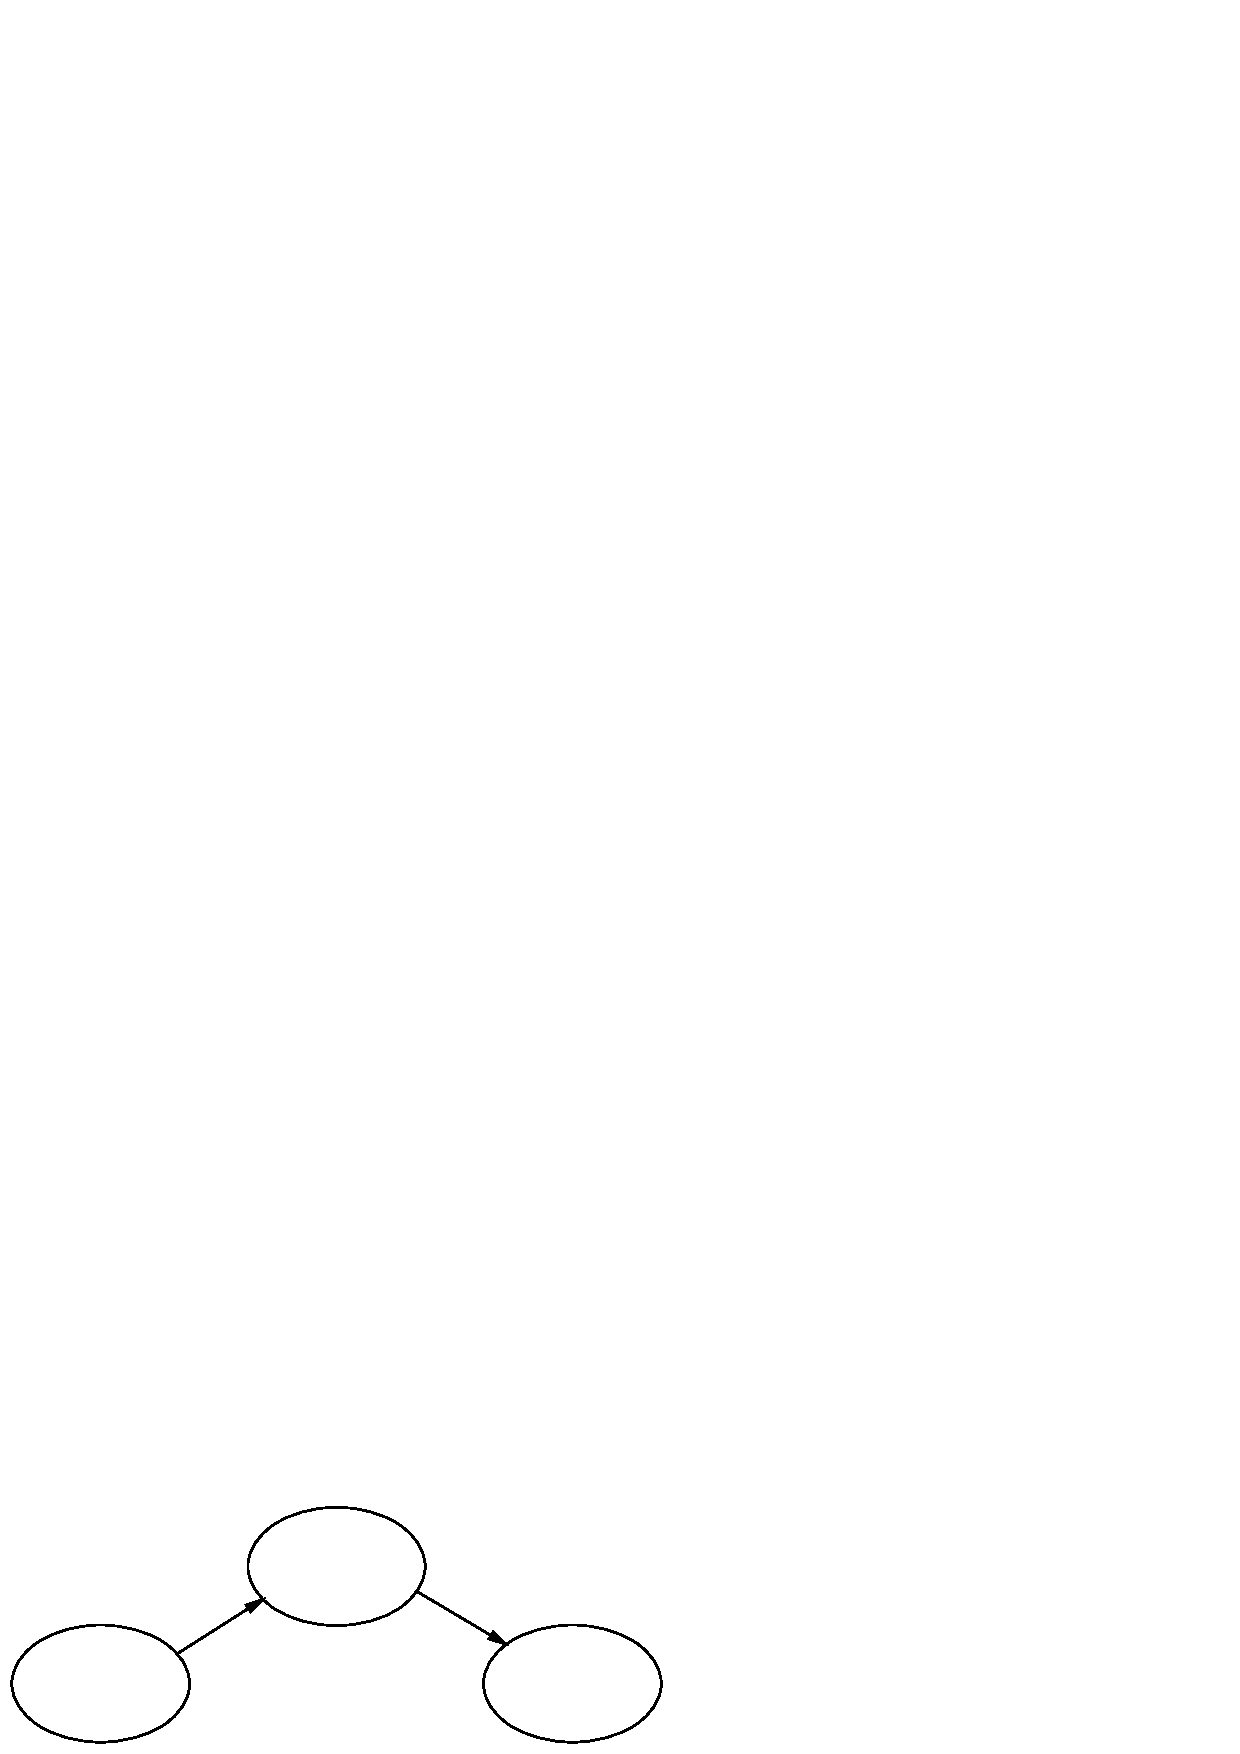
\includegraphics[width=200px]{gfx/pub_sub.png}
	\caption{publish subsribe system}
	\label{img:publish_subscribe}
\end{figure}
\item processes communicates threough events
\item publisher announces events at broker\\
$\Rightarrow$ loose coupling (publisher and subscriber need not to know each other), decoupled in space\\
$\Rightarrow$ scalability better than client-server, parallel processing, caching\\
\end{itemize}
Event-based and data-based can be combined\\
$\Rightarrow$ shared Data space \\
\begin{figure}
	\centering
	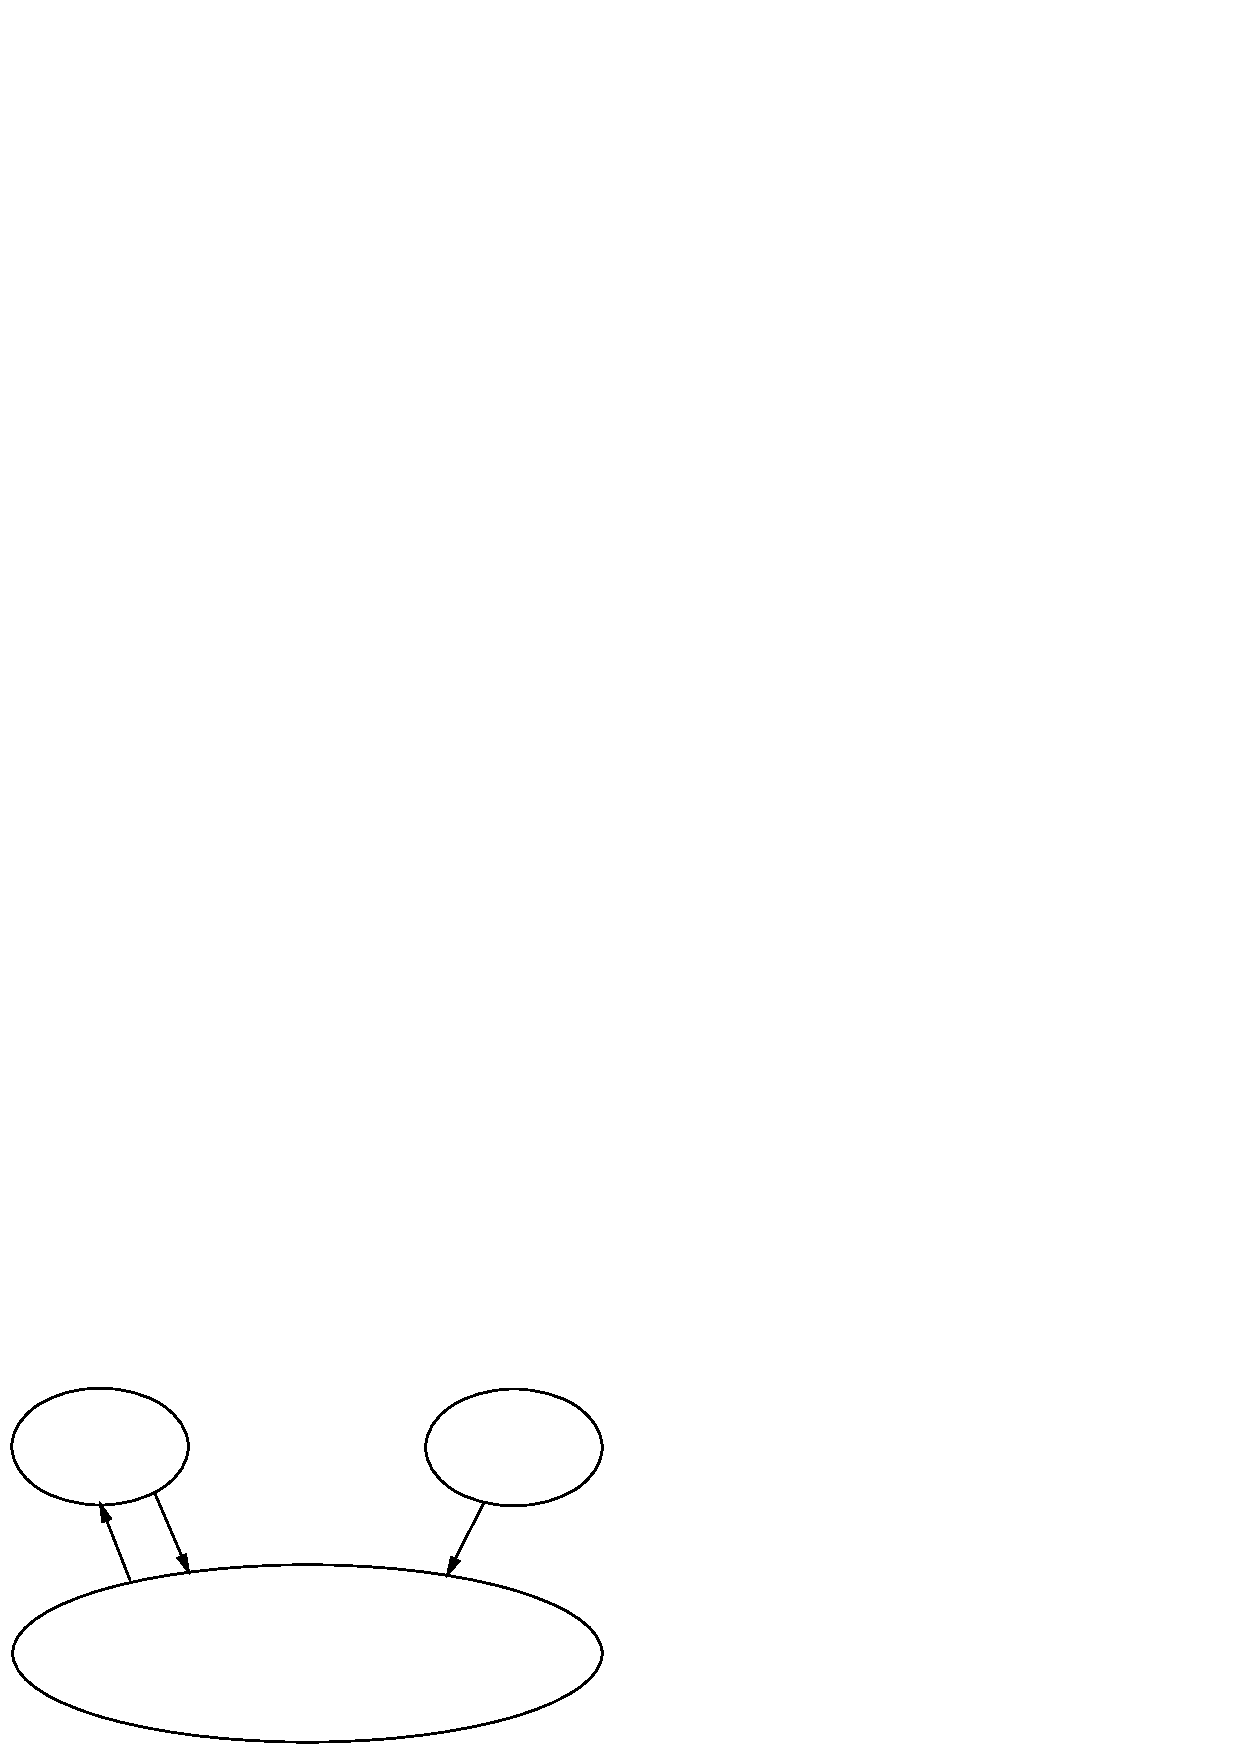
\includegraphics[width=200px]{gfx/shared_data_space.png}
	\caption{shared data space}
	\label{img:shared_data_space}
\end{figure}
\end{itemize}

\subsection{System architectures}
\begin{enummerate}
\item centralized architectures\\
client - server\\
\begin{itemize}
\item[(i)] single point of failure
\item[(ii)] performance (server is bottleneck)\\
\begin{figure}
	\centering
	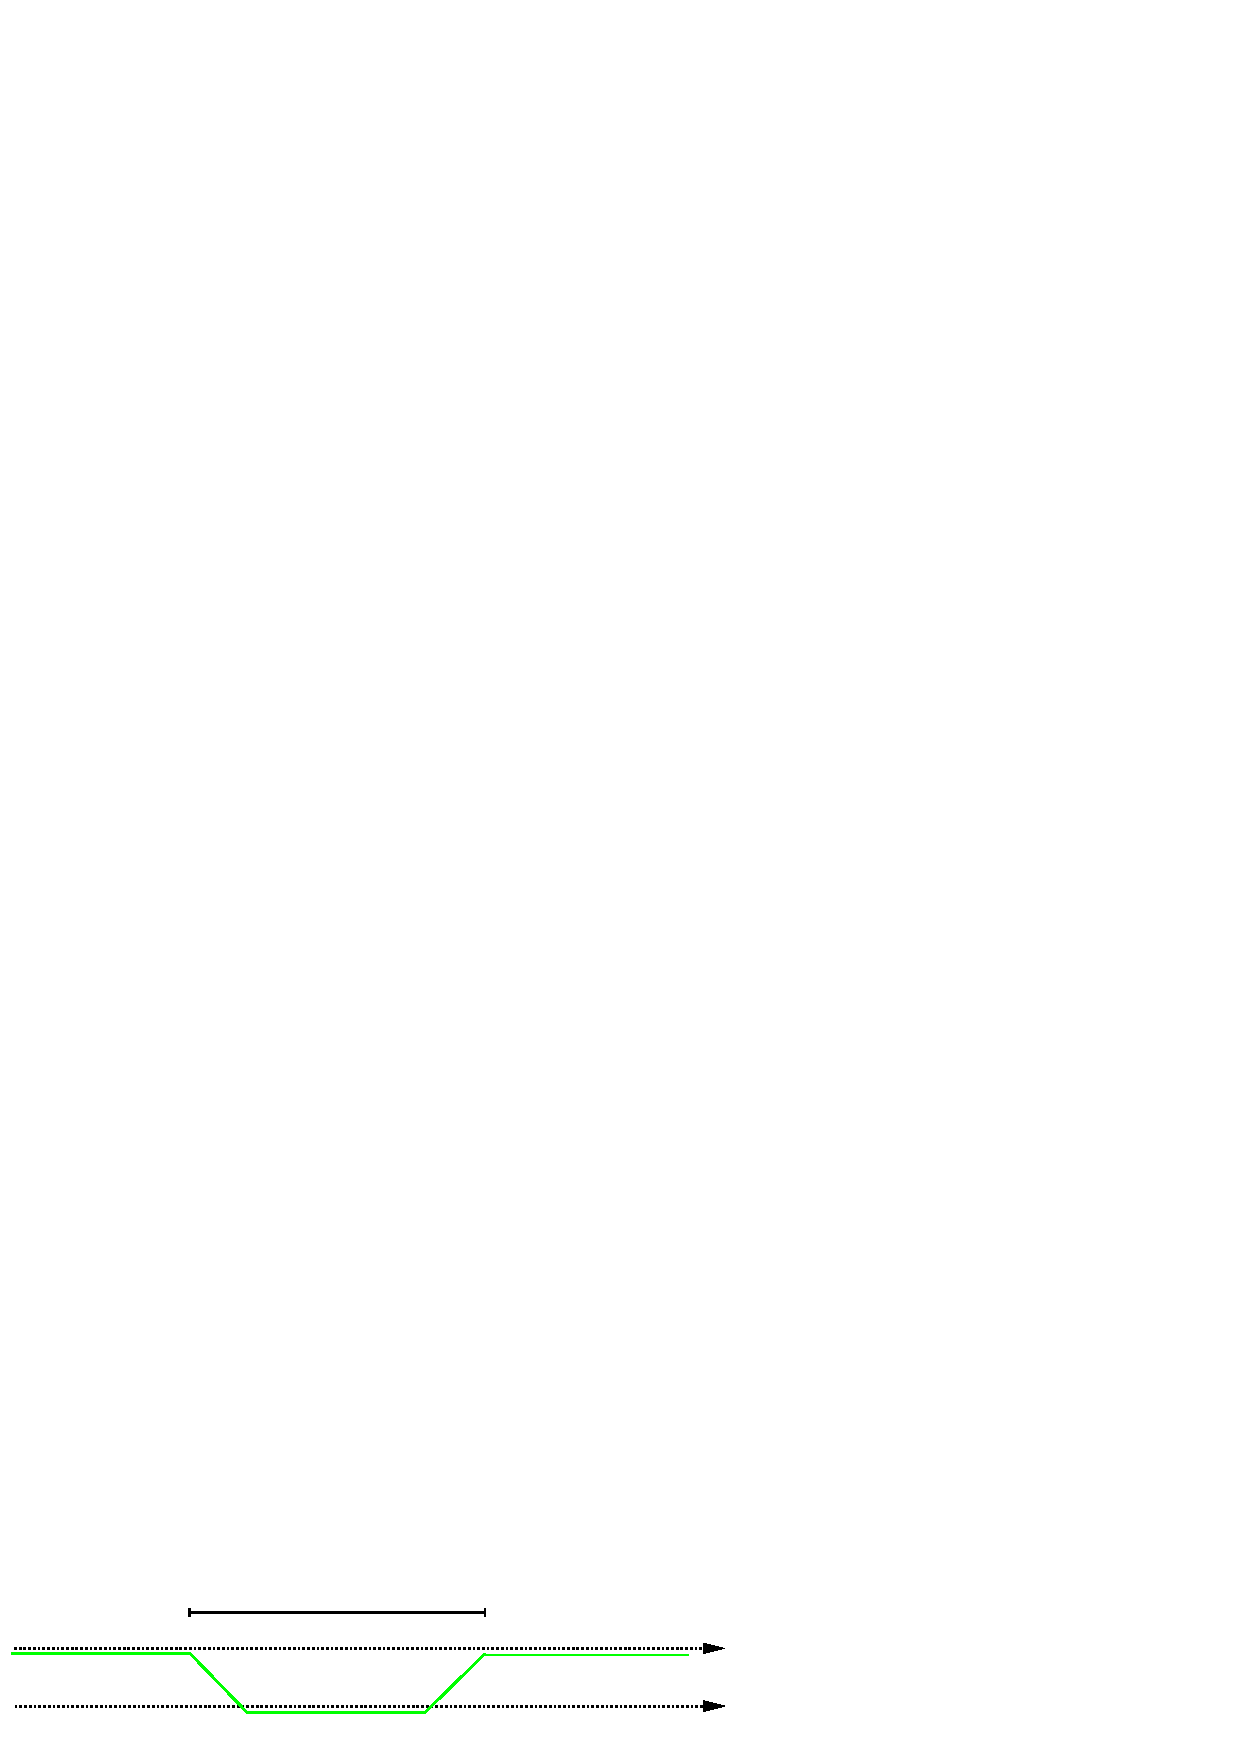
\includegraphics[width=200px]{gfx/cs_simple_wait.png}
	\caption{client server simple waiting situation}
	\label{img:cs_simple_wait}
\end{figure}
\begin{enumerate}
\item communication problems\\
\item server problems\\
\end{enumerate}
can request be repeated without harm?\\
$\Rightarrow$ request is idempotent
\item[(iii)] aplication layering\\
Layers:\begin{itemize}
\item[1.)] User interface
\item[2.)] processing
\item[3.)] data level
\begin{figure}
	\centering
	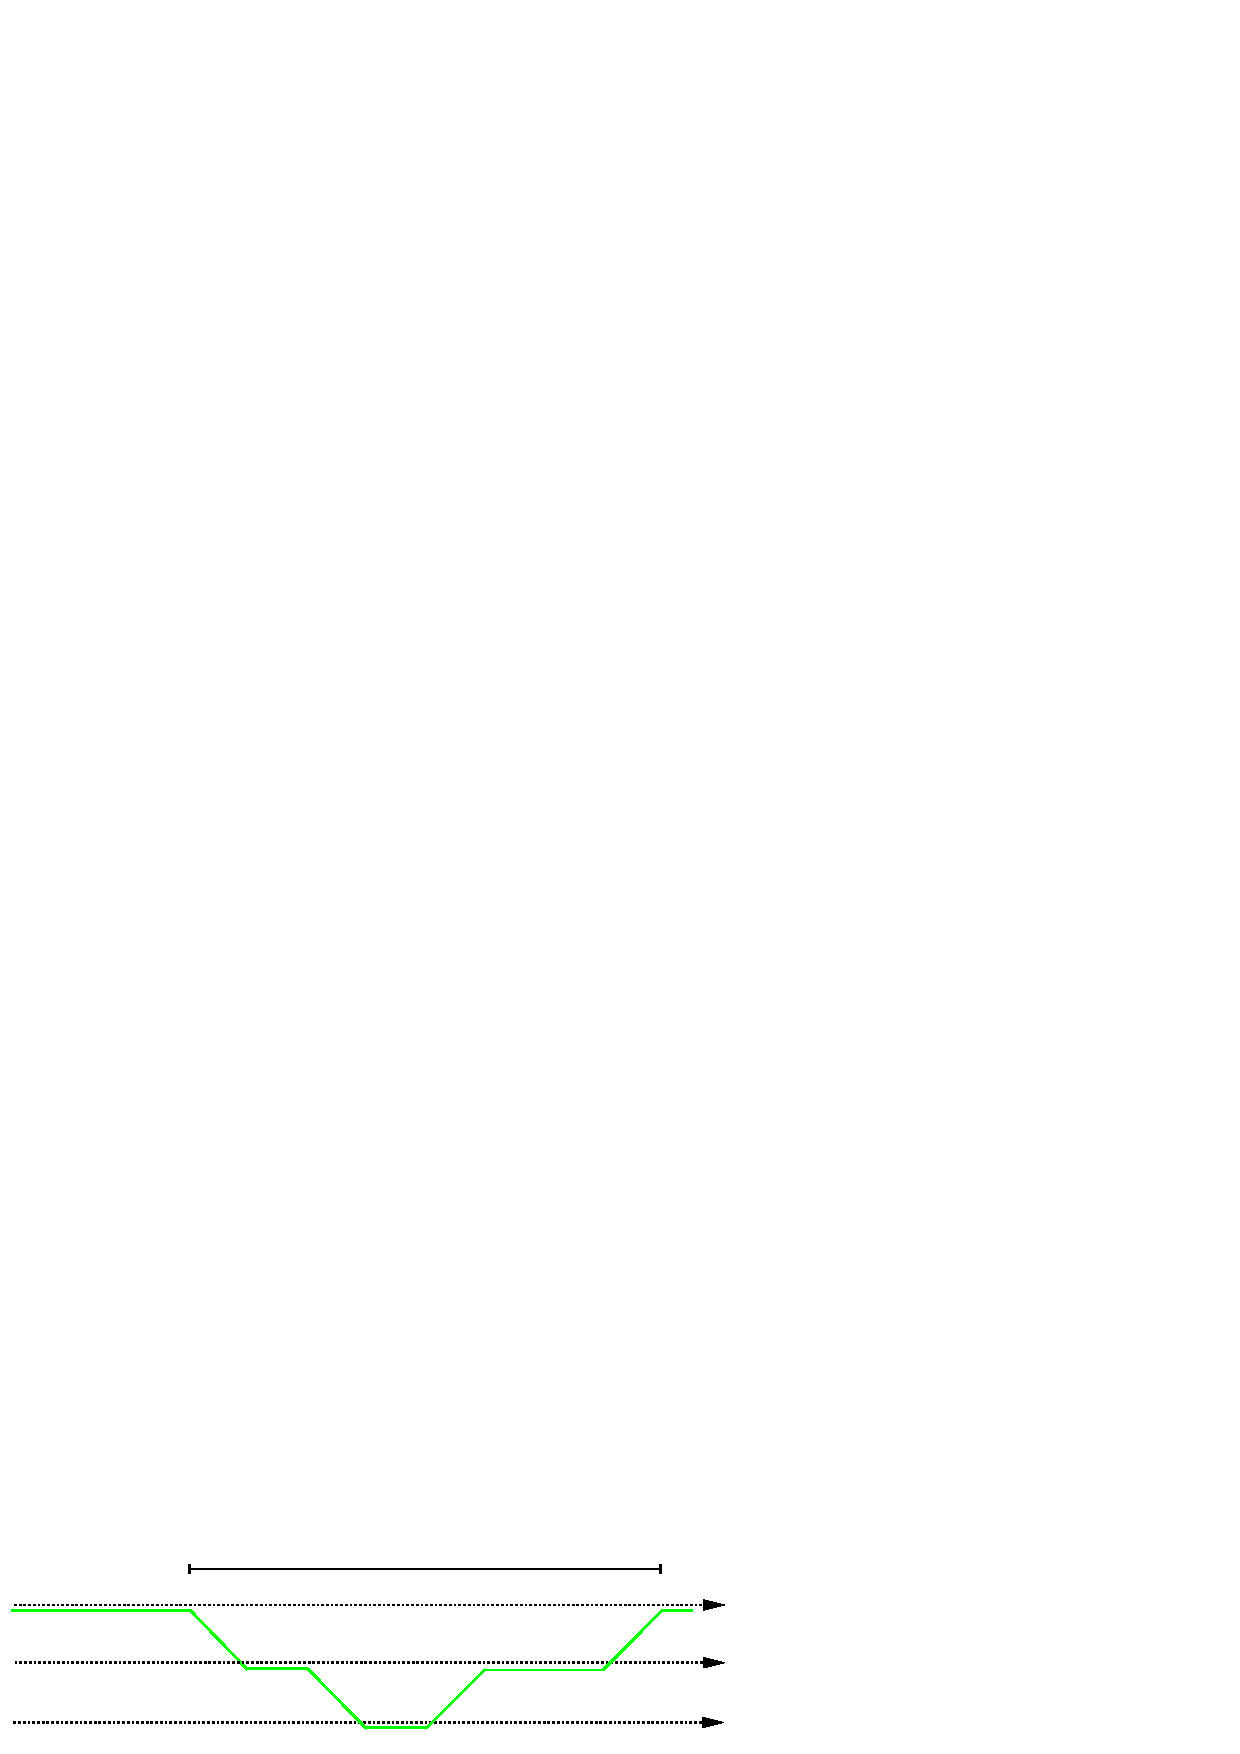
\includegraphics[width=200px]{gfx/cs_app_layer.png}
	\caption{application layer}
	\label{img:cs_app_layer}
\end{figure}
\end{itemize}
$\Rightarrow$ a lot of waiting\\
$\Rightarrow$ does not scale\\
\end{itemize}
\item Decentralized architectures\\
\begin{ itemize}
\item vertical distribution (layering)\\
different logic on different machines
\item horizontal distribution \\
replicated client/server operating on different data\\
$\Rightarrow$ overlay-underlay hides physical structure by adding logical structure\\
\end{itemize}

Structured P2P architectures\\
\begin{itemize}
\item most popular technique is distributed hashtables (DHT)\\
\item randomly 128 bit or 160 bit ke for data and nodes. Two or more keys are very unlikely\\
\item Chord system arranges items in a ring 
\item data item k is assigened to node with smallest identifier id $\geq$ k
\end{itemize}
ie item 1 belongs to node 1\\
item 2 belongs to node 2\\
for each item k$_i$ succ(k)=id\\
returns  the name of the node k is assigened to\\
to find data item k the function LOOKUP(k) returns the adress of succ(k) in O(log(N)(later!)\\

membership management\\
join:\\
create SHA1 identifier\\
LOOKUP(id) = succ(id)\\
contact succ(id) and pred(id) to join ring\\

leave:\\
node id informs succ(id) and pred(id) and assigns it's data to succ(id)\\

Content adressable network (CAN)\\
\begin{itemize}
\item d-dimensional cartesian space
\item every node draws random number
\item space is divided among nodes
\item every data draws identifier (coodinates) which assigns a node

\item join\begin{itemize}
\item select random point
\item half the square in which id falls
\item assign item to centers
\end{itemize}
\item leave\begin{itemize}
\item one node takes the rectangle\\
$\Rightarrow$ reassign rectangles periodically
\end{itemize}
\end{itemize}

Unstructured P2P Network\\
\begin{itemize}
\item random graph
\item each node maintains a list of c neighbours
\item partial view or neighbourhood list  with age
\item nodes exchange neighbour information \\active thread\\ select peer\\

PUSH\\
select c/2 youngest entries+myself\\
send to peer\\

PULL\\
receive peer buffer\\
construct new partial view\\
increment age\\

passive thread\\
recieve buffer from peer\\

PULL:\\
select c/2\\
send to peer\\
construct new partial view
increment age\\

\end{itemize}

\end{enummerate}


\end{document}
